\documentclass[12pt]{article}
\usepackage{tikz}
\usepackage{amsmath}
% Underlining package
\usepackage{ulem}
\usetikzlibrary{calc}
\usepackage[a4paper, portrait, margin=1cm]{geometry}
\usepackage{fancyhdr}

\def \HeadingQuestions {\section*{\Large Name: \underline{\hspace{8cm}} \hfill Date: \underline{\hspace{3cm}}} \vspace{-3mm}
{Angles in Right Triangles: Questions} \vspace{1pt}\hrule}

% raise footer with page number; no header
\fancypagestyle{myfancypagestyle}{
  \fancyhf{}% clear all header and footer fields
  \renewcommand{\headrulewidth}{0pt} % no rule under header
  \fancyfoot[C] {\thepage} \setlength{\footskip}{14.5pt} % raise page number 6pt
}
\pagestyle{myfancypagestyle}  % apply myfancypagestyle

\newcounter{minipagecount}

\begin{document}
\HeadingQuestions
\vspace{8mm}

\begin{minipage}{0.55\textwidth}
  \refstepcounter{minipagecount}
  \noindent{(\theminipagecount)}\quad
  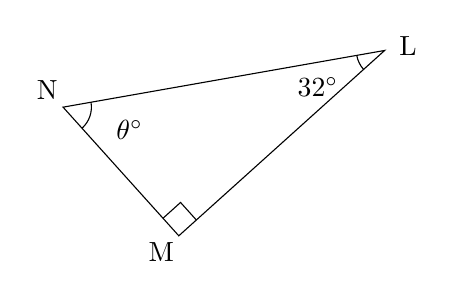
\begin{tikzpicture}[scale=1.2, baseline=(current bounding box.north)]

    \begin{scope}[rotate=190]
      \coordinate (A) at (0,0);
      \coordinate (B) at (3.4554400438163886,0);
      \coordinate (C) at (intersection cs: first line={(A)--($(A)+(32:4cm)$)}, second line={(B)--($(B)+(180-58:4cm)$)});
      \draw (A) -- (B) -- (C) -- cycle;

      % Mark angles with arcs
      \draw ($(A)!0.3cm!(B)$) arc [start angle=0, end angle=32, radius=0.3cm];
      \draw ($(B)!0.3cm!(C)$) arc [start angle=180-58, end angle=180, radius=0.3cm];
      % \draw ($(C)!0.3cm!(A)$) arc [start angle=180+32, end angle=360-58, radius=0.3cm];
      % rt angle mark at C
      % \tkzMarkRightAng0le(A,C,B); % uses \usepackage{tkz-euclide}
      \draw ($(C)!0.25cm!(A)$) -- ($(C)!0.25cm!(A)!0.25cm!90:(A)$) -- ($(C)!0.25cm!(B)$);
      %  The ($(C)!0.3cm!(A)!0.3cm!90:(A)$) syntax is used to specify a point that is 0.3cm away from the point ($(C)!0.3cm!(A)$) in a direction that is perpendicular to the line connecting points C and A. This is achieved by first specifying the point ($(C)!0.3cm!(A)$) and then rotating it by 90 degrees around point A using the !angle:anchor syntax.

      % Label angles
      \node at ($(A)!-0.25cm!(B)$) {L};
      \node at ($(B)!-0.25cm!(C)$) {N};
      \node at ($(C)!-0.25cm!(A)$) {M};

      % Mark angles in degrees
      \coordinate (midBC) at ($(B)!0.5!(C)$);
      \node at ($(A)!0.665cm!(midBC)!0.15cm!(C)$) {$32^\circ$};

      \coordinate (midAC) at ($(A)!0.5!(C)$);
      \node at ($(B)!0.65cm!(midAC)!0.15cm!(C)$) {$\theta^\circ$};

      % \coordinate (midAB) at ($(A)!0.5!(B)$);
      % \node at ($(C)!0.55cm!(midAB)$) {<<angleCValueDisplay>>$^\circ$};

    \end{scope}
  \end{tikzpicture}
\end{minipage}%
\hfill
\begin{minipage}{0.4\textwidth}
  \begin{align*}
    \theta^\circ &= 90^\circ - \angle \text{\dotuline{~~~~~~~}} \\
    &= 90^\circ - \dotuline{~~~~~~~}^\circ  \\
    &= \dotuline{~~~~~~~}^\circ
  \end{align*}
\end{minipage}
\vspace{1cm}\begin{minipage}{0.55\textwidth}
  \refstepcounter{minipagecount}
  \noindent{(\theminipagecount)}\quad
  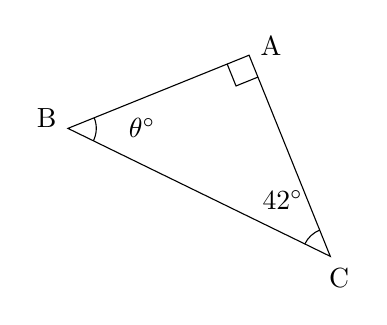
\begin{tikzpicture}[scale=1.2, baseline=(current bounding box.north)]

    \begin{scope}[rotate=334]
      \coordinate (A) at (0,0);
      \coordinate (B) at (3.089134642379471,0);
      \coordinate (C) at (intersection cs: first line={(A)--($(A)+(48:4cm)$)}, second line={(B)--($(B)+(180-42:4cm)$)});
      \draw (A) -- (B) -- (C) -- cycle;

      % Mark angles with arcs
      \draw ($(A)!0.3cm!(B)$) arc [start angle=0, end angle=48, radius=0.3cm];
      \draw ($(B)!0.3cm!(C)$) arc [start angle=180-42, end angle=180, radius=0.3cm];
      % \draw ($(C)!0.3cm!(A)$) arc [start angle=180+48, end angle=360-42, radius=0.3cm];
      % rt angle mark at C
      % \tkzMarkRightAng0le(A,C,B); % uses \usepackage{tkz-euclide}
      \draw ($(C)!0.25cm!(A)$) -- ($(C)!0.25cm!(A)!0.25cm!90:(A)$) -- ($(C)!0.25cm!(B)$);
      %  The ($(C)!0.3cm!(A)!0.3cm!90:(A)$) syntax is used to specify a point that is 0.3cm away from the point ($(C)!0.3cm!(A)$) in a direction that is perpendicular to the line connecting points C and A. This is achieved by first specifying the point ($(C)!0.3cm!(A)$) and then rotating it by 90 degrees around point A using the !angle:anchor syntax.

      % Label angles
      \node at ($(A)!-0.25cm!(B)$) {B};
      \node at ($(B)!-0.25cm!(C)$) {C};
      \node at ($(C)!-0.25cm!(A)$) {A};

      % Mark angles in degrees
      \coordinate (midBC) at ($(B)!0.5!(C)$);
      \node at ($(A)!0.665cm!(midBC)!0.15cm!(C)$) {$\theta^\circ$};

      \coordinate (midAC) at ($(A)!0.5!(C)$);
      \node at ($(B)!0.65cm!(midAC)!0.15cm!(C)$) {$42^\circ$};

      % \coordinate (midAB) at ($(A)!0.5!(B)$);
      % \node at ($(C)!0.55cm!(midAB)$) {<<angleCValueDisplay>>$^\circ$};

    \end{scope}
  \end{tikzpicture}
\end{minipage}%
\hfill
\begin{minipage}{0.4\textwidth}
  \begin{align*}
    \theta^\circ &= 90^\circ - \angle \text{\dotuline{~~~~~~~}} \\
    &= 90^\circ - \dotuline{~~~~~~~}^\circ  \\
    &= \dotuline{~~~~~~~}^\circ
  \end{align*}
\end{minipage}
\vspace{1cm}\begin{minipage}{0.55\textwidth}
  \refstepcounter{minipagecount}
  \noindent{(\theminipagecount)}\quad
  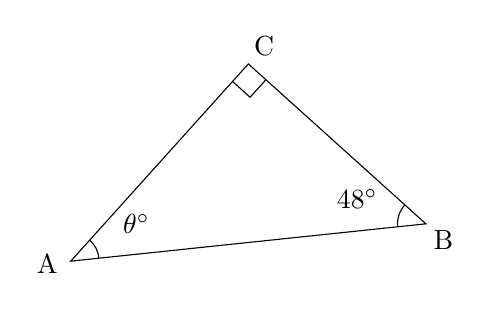
\begin{tikzpicture}[scale=1.2, baseline=(current bounding box.north)]

    \begin{scope}[rotate=6]
      \coordinate (A) at (0,0);
      \coordinate (B) at (3.7782832605581795,0);
      \coordinate (C) at (intersection cs: first line={(A)--($(A)+(42:4cm)$)}, second line={(B)--($(B)+(180-48:4cm)$)});
      \draw (A) -- (B) -- (C) -- cycle;

      % Mark angles with arcs
      \draw ($(A)!0.3cm!(B)$) arc [start angle=0, end angle=42, radius=0.3cm];
      \draw ($(B)!0.3cm!(C)$) arc [start angle=180-48, end angle=180, radius=0.3cm];
      % \draw ($(C)!0.3cm!(A)$) arc [start angle=180+42, end angle=360-48, radius=0.3cm];
      % rt angle mark at C
      % \tkzMarkRightAng0le(A,C,B); % uses \usepackage{tkz-euclide}
      \draw ($(C)!0.25cm!(A)$) -- ($(C)!0.25cm!(A)!0.25cm!90:(A)$) -- ($(C)!0.25cm!(B)$);
      %  The ($(C)!0.3cm!(A)!0.3cm!90:(A)$) syntax is used to specify a point that is 0.3cm away from the point ($(C)!0.3cm!(A)$) in a direction that is perpendicular to the line connecting points C and A. This is achieved by first specifying the point ($(C)!0.3cm!(A)$) and then rotating it by 90 degrees around point A using the !angle:anchor syntax.

      % Label angles
      \node at ($(A)!-0.25cm!(B)$) {A};
      \node at ($(B)!-0.25cm!(C)$) {B};
      \node at ($(C)!-0.25cm!(A)$) {C};

      % Mark angles in degrees
      \coordinate (midBC) at ($(B)!0.5!(C)$);
      \node at ($(A)!0.665cm!(midBC)!0.15cm!(C)$) {$\theta^\circ$};

      \coordinate (midAC) at ($(A)!0.5!(C)$);
      \node at ($(B)!0.65cm!(midAC)!0.15cm!(C)$) {$48^\circ$};

      % \coordinate (midAB) at ($(A)!0.5!(B)$);
      % \node at ($(C)!0.55cm!(midAB)$) {<<angleCValueDisplay>>$^\circ$};

    \end{scope}
  \end{tikzpicture}
\end{minipage}%
\hfill
\begin{minipage}{0.4\textwidth}
  \begin{align*}
    \theta^\circ &= 90^\circ - \angle \text{\dotuline{~~~~~~~}} \\
    &= 90^\circ - \dotuline{~~~~~~~}^\circ  \\
    &= \dotuline{~~~~~~~}^\circ
  \end{align*}
\end{minipage}
\vspace{1cm}\begin{minipage}{0.55\textwidth}
  \refstepcounter{minipagecount}
  \noindent{(\theminipagecount)}\quad
  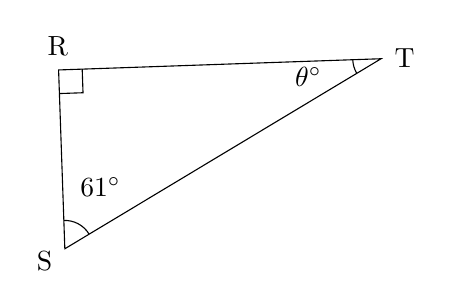
\begin{tikzpicture}[scale=1.2, baseline=(current bounding box.north)]

    \begin{scope}[rotate=31]
      \coordinate (A) at (0,0);
      \coordinate (B) at (3.9043741352637564,0);
      \coordinate (C) at (intersection cs: first line={(A)--($(A)+(61:4cm)$)}, second line={(B)--($(B)+(180-29:4cm)$)});
      \draw (A) -- (B) -- (C) -- cycle;

      % Mark angles with arcs
      \draw ($(A)!0.3cm!(B)$) arc [start angle=0, end angle=61, radius=0.3cm];
      \draw ($(B)!0.3cm!(C)$) arc [start angle=180-29, end angle=180, radius=0.3cm];
      % \draw ($(C)!0.3cm!(A)$) arc [start angle=180+61, end angle=360-29, radius=0.3cm];
      % rt angle mark at C
      % \tkzMarkRightAng0le(A,C,B); % uses \usepackage{tkz-euclide}
      \draw ($(C)!0.25cm!(A)$) -- ($(C)!0.25cm!(A)!0.25cm!90:(A)$) -- ($(C)!0.25cm!(B)$);
      %  The ($(C)!0.3cm!(A)!0.3cm!90:(A)$) syntax is used to specify a point that is 0.3cm away from the point ($(C)!0.3cm!(A)$) in a direction that is perpendicular to the line connecting points C and A. This is achieved by first specifying the point ($(C)!0.3cm!(A)$) and then rotating it by 90 degrees around point A using the !angle:anchor syntax.

      % Label angles
      \node at ($(A)!-0.25cm!(B)$) {S};
      \node at ($(B)!-0.25cm!(C)$) {T};
      \node at ($(C)!-0.25cm!(A)$) {R};

      % Mark angles in degrees
      \coordinate (midBC) at ($(B)!0.5!(C)$);
      \node at ($(A)!0.665cm!(midBC)!0.15cm!(C)$) {$61^\circ$};

      \coordinate (midAC) at ($(A)!0.5!(C)$);
      \node at ($(B)!0.65cm!(midAC)!0.15cm!(C)$) {$\theta^\circ$};

      % \coordinate (midAB) at ($(A)!0.5!(B)$);
      % \node at ($(C)!0.55cm!(midAB)$) {<<angleCValueDisplay>>$^\circ$};

    \end{scope}
  \end{tikzpicture}
\end{minipage}%
\hfill
\begin{minipage}{0.4\textwidth}
  \begin{align*}
    \theta^\circ &= 90^\circ - \angle \text{\dotuline{~~~~~~~}} \\
    &= 90^\circ - \dotuline{~~~~~~~}^\circ  \\
    &= \dotuline{~~~~~~~}^\circ
  \end{align*}
\end{minipage}
\vspace{1cm}\begin{minipage}{0.55\textwidth}
  \refstepcounter{minipagecount}
  \noindent{(\theminipagecount)}\quad
  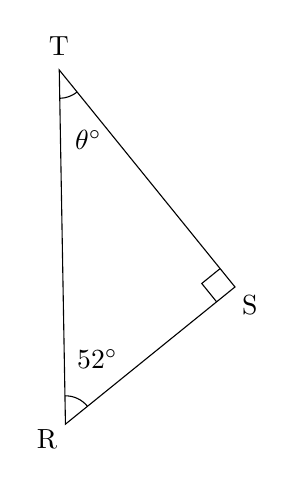
\begin{tikzpicture}[scale=1.2, baseline=(current bounding box.north)]

    \begin{scope}[rotate=271]
      \coordinate (A) at (0,0);
      \coordinate (B) at (3.748231175110153,0);
      \coordinate (C) at (intersection cs: first line={(A)--($(A)+(38:4cm)$)}, second line={(B)--($(B)+(180-52:4cm)$)});
      \draw (A) -- (B) -- (C) -- cycle;

      % Mark angles with arcs
      \draw ($(A)!0.3cm!(B)$) arc [start angle=0, end angle=38, radius=0.3cm];
      \draw ($(B)!0.3cm!(C)$) arc [start angle=180-52, end angle=180, radius=0.3cm];
      % \draw ($(C)!0.3cm!(A)$) arc [start angle=180+38, end angle=360-52, radius=0.3cm];
      % rt angle mark at C
      % \tkzMarkRightAng0le(A,C,B); % uses \usepackage{tkz-euclide}
      \draw ($(C)!0.25cm!(A)$) -- ($(C)!0.25cm!(A)!0.25cm!90:(A)$) -- ($(C)!0.25cm!(B)$);
      %  The ($(C)!0.3cm!(A)!0.3cm!90:(A)$) syntax is used to specify a point that is 0.3cm away from the point ($(C)!0.3cm!(A)$) in a direction that is perpendicular to the line connecting points C and A. This is achieved by first specifying the point ($(C)!0.3cm!(A)$) and then rotating it by 90 degrees around point A using the !angle:anchor syntax.

      % Label angles
      \node at ($(A)!-0.25cm!(B)$) {T};
      \node at ($(B)!-0.25cm!(C)$) {R};
      \node at ($(C)!-0.25cm!(A)$) {S};

      % Mark angles in degrees
      \coordinate (midBC) at ($(B)!0.5!(C)$);
      \node at ($(A)!0.665cm!(midBC)!0.15cm!(C)$) {$\theta^\circ$};

      \coordinate (midAC) at ($(A)!0.5!(C)$);
      \node at ($(B)!0.65cm!(midAC)!0.15cm!(C)$) {$52^\circ$};

      % \coordinate (midAB) at ($(A)!0.5!(B)$);
      % \node at ($(C)!0.55cm!(midAB)$) {<<angleCValueDisplay>>$^\circ$};

    \end{scope}
  \end{tikzpicture}
\end{minipage}%
\hfill
\begin{minipage}{0.4\textwidth}
  \begin{align*}
    \theta^\circ &= 90^\circ - \angle \text{\dotuline{~~~~~~~}} \\
    &= 90^\circ - \dotuline{~~~~~~~}^\circ  \\
    &= \dotuline{~~~~~~~}^\circ
  \end{align*}
\end{minipage}
\vspace{1cm}\begin{minipage}{0.55\textwidth}
  \refstepcounter{minipagecount}
  \noindent{(\theminipagecount)}\quad
  \begin{tikzpicture}[scale=1.2, baseline=(current bounding box.north)]

    \begin{scope}[rotate=323]
      \coordinate (A) at (0,0);
      \coordinate (B) at (3.8115408961805817,0);
      \coordinate (C) at (intersection cs: first line={(A)--($(A)+(62:4cm)$)}, second line={(B)--($(B)+(180-28:4cm)$)});
      \draw (A) -- (B) -- (C) -- cycle;

      % Mark angles with arcs
      \draw ($(A)!0.3cm!(B)$) arc [start angle=0, end angle=62, radius=0.3cm];
      \draw ($(B)!0.3cm!(C)$) arc [start angle=180-28, end angle=180, radius=0.3cm];
      % \draw ($(C)!0.3cm!(A)$) arc [start angle=180+62, end angle=360-28, radius=0.3cm];
      % rt angle mark at C
      % \tkzMarkRightAng0le(A,C,B); % uses \usepackage{tkz-euclide}
      \draw ($(C)!0.25cm!(A)$) -- ($(C)!0.25cm!(A)!0.25cm!90:(A)$) -- ($(C)!0.25cm!(B)$);
      %  The ($(C)!0.3cm!(A)!0.3cm!90:(A)$) syntax is used to specify a point that is 0.3cm away from the point ($(C)!0.3cm!(A)$) in a direction that is perpendicular to the line connecting points C and A. This is achieved by first specifying the point ($(C)!0.3cm!(A)$) and then rotating it by 90 degrees around point A using the !angle:anchor syntax.

      % Label angles
      \node at ($(A)!-0.25cm!(B)$) {X};
      \node at ($(B)!-0.25cm!(C)$) {Y};
      \node at ($(C)!-0.25cm!(A)$) {Z};

      % Mark angles in degrees
      \coordinate (midBC) at ($(B)!0.5!(C)$);
      \node at ($(A)!0.665cm!(midBC)!0.15cm!(C)$) {$62^\circ$};

      \coordinate (midAC) at ($(A)!0.5!(C)$);
      \node at ($(B)!0.65cm!(midAC)!0.15cm!(C)$) {$\theta^\circ$};

      % \coordinate (midAB) at ($(A)!0.5!(B)$);
      % \node at ($(C)!0.55cm!(midAB)$) {<<angleCValueDisplay>>$^\circ$};

    \end{scope}
  \end{tikzpicture}
\end{minipage}%
\hfill
\begin{minipage}{0.4\textwidth}
  \begin{align*}
    \theta^\circ &= 90^\circ - \angle \text{\dotuline{~~~~~~~}} \\
    &= 90^\circ - \dotuline{~~~~~~~}^\circ  \\
    &= \dotuline{~~~~~~~}^\circ
  \end{align*}
\end{minipage}
\vspace{1cm}\begin{minipage}{0.55\textwidth}
  \refstepcounter{minipagecount}
  \noindent{(\theminipagecount)}\quad
  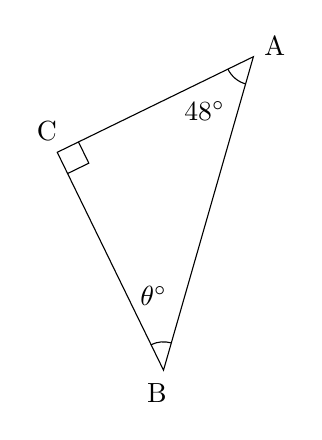
\begin{tikzpicture}[scale=1.2, baseline=(current bounding box.north)]

    \begin{scope}[rotate=74]
      \coordinate (A) at (0,0);
      \coordinate (B) at (3.4508781443189167,0);
      \coordinate (C) at (intersection cs: first line={(A)--($(A)+(42:4cm)$)}, second line={(B)--($(B)+(180-48:4cm)$)});
      \draw (A) -- (B) -- (C) -- cycle;

      % Mark angles with arcs
      \draw ($(A)!0.3cm!(B)$) arc [start angle=0, end angle=42, radius=0.3cm];
      \draw ($(B)!0.3cm!(C)$) arc [start angle=180-48, end angle=180, radius=0.3cm];
      % \draw ($(C)!0.3cm!(A)$) arc [start angle=180+42, end angle=360-48, radius=0.3cm];
      % rt angle mark at C
      % \tkzMarkRightAng0le(A,C,B); % uses \usepackage{tkz-euclide}
      \draw ($(C)!0.25cm!(A)$) -- ($(C)!0.25cm!(A)!0.25cm!90:(A)$) -- ($(C)!0.25cm!(B)$);
      %  The ($(C)!0.3cm!(A)!0.3cm!90:(A)$) syntax is used to specify a point that is 0.3cm away from the point ($(C)!0.3cm!(A)$) in a direction that is perpendicular to the line connecting points C and A. This is achieved by first specifying the point ($(C)!0.3cm!(A)$) and then rotating it by 90 degrees around point A using the !angle:anchor syntax.

      % Label angles
      \node at ($(A)!-0.25cm!(B)$) {B};
      \node at ($(B)!-0.25cm!(C)$) {A};
      \node at ($(C)!-0.25cm!(A)$) {C};

      % Mark angles in degrees
      \coordinate (midBC) at ($(B)!0.5!(C)$);
      \node at ($(A)!0.665cm!(midBC)!0.15cm!(C)$) {$\theta^\circ$};

      \coordinate (midAC) at ($(A)!0.5!(C)$);
      \node at ($(B)!0.65cm!(midAC)!0.15cm!(C)$) {$48^\circ$};

      % \coordinate (midAB) at ($(A)!0.5!(B)$);
      % \node at ($(C)!0.55cm!(midAB)$) {<<angleCValueDisplay>>$^\circ$};

    \end{scope}
  \end{tikzpicture}
\end{minipage}%
\hfill
\begin{minipage}{0.4\textwidth}
  \begin{align*}
    \theta^\circ &= 90^\circ - \angle \text{\dotuline{~~~~~~~}} \\
    &= 90^\circ - \dotuline{~~~~~~~}^\circ  \\
    &= \dotuline{~~~~~~~}^\circ
  \end{align*}
\end{minipage}
\vspace{1cm}\begin{minipage}{0.55\textwidth}
  \refstepcounter{minipagecount}
  \noindent{(\theminipagecount)}\quad
  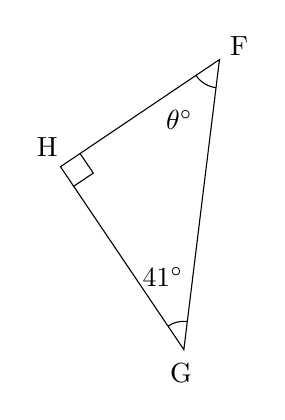
\begin{tikzpicture}[scale=1.2, baseline=(current bounding box.north)]

    \begin{scope}[rotate=83]
      \coordinate (A) at (0,0);
      \coordinate (B) at (3.0925086998760096,0);
      \coordinate (C) at (intersection cs: first line={(A)--($(A)+(41:4cm)$)}, second line={(B)--($(B)+(180-49:4cm)$)});
      \draw (A) -- (B) -- (C) -- cycle;

      % Mark angles with arcs
      \draw ($(A)!0.3cm!(B)$) arc [start angle=0, end angle=41, radius=0.3cm];
      \draw ($(B)!0.3cm!(C)$) arc [start angle=180-49, end angle=180, radius=0.3cm];
      % \draw ($(C)!0.3cm!(A)$) arc [start angle=180+41, end angle=360-49, radius=0.3cm];
      % rt angle mark at C
      % \tkzMarkRightAng0le(A,C,B); % uses \usepackage{tkz-euclide}
      \draw ($(C)!0.25cm!(A)$) -- ($(C)!0.25cm!(A)!0.25cm!90:(A)$) -- ($(C)!0.25cm!(B)$);
      %  The ($(C)!0.3cm!(A)!0.3cm!90:(A)$) syntax is used to specify a point that is 0.3cm away from the point ($(C)!0.3cm!(A)$) in a direction that is perpendicular to the line connecting points C and A. This is achieved by first specifying the point ($(C)!0.3cm!(A)$) and then rotating it by 90 degrees around point A using the !angle:anchor syntax.

      % Label angles
      \node at ($(A)!-0.25cm!(B)$) {G};
      \node at ($(B)!-0.25cm!(C)$) {F};
      \node at ($(C)!-0.25cm!(A)$) {H};

      % Mark angles in degrees
      \coordinate (midBC) at ($(B)!0.5!(C)$);
      \node at ($(A)!0.665cm!(midBC)!0.15cm!(C)$) {$41^\circ$};

      \coordinate (midAC) at ($(A)!0.5!(C)$);
      \node at ($(B)!0.65cm!(midAC)!0.15cm!(C)$) {$\theta^\circ$};

      % \coordinate (midAB) at ($(A)!0.5!(B)$);
      % \node at ($(C)!0.55cm!(midAB)$) {<<angleCValueDisplay>>$^\circ$};

    \end{scope}
  \end{tikzpicture}
\end{minipage}%
\hfill
\begin{minipage}{0.4\textwidth}
  \begin{align*}
    \theta^\circ &= 90^\circ - \angle \text{\dotuline{~~~~~~~}} \\
    &= 90^\circ - \dotuline{~~~~~~~}^\circ  \\
    &= \dotuline{~~~~~~~}^\circ
  \end{align*}
\end{minipage}
\vspace{1cm}\begin{minipage}{0.55\textwidth}
  \refstepcounter{minipagecount}
  \noindent{(\theminipagecount)}\quad
  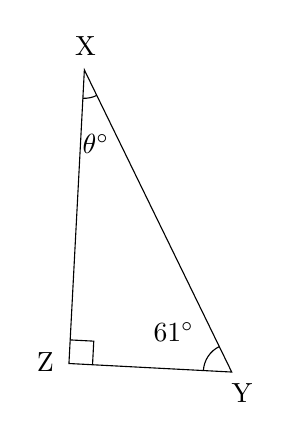
\begin{tikzpicture}[scale=1.2, baseline=(current bounding box.north)]

    \begin{scope}[rotate=116]
      \coordinate (A) at (0,0);
      \coordinate (B) at (3.556837432041295,0);
      \coordinate (C) at (intersection cs: first line={(A)--($(A)+(61:4cm)$)}, second line={(B)--($(B)+(180-29:4cm)$)});
      \draw (A) -- (B) -- (C) -- cycle;

      % Mark angles with arcs
      \draw ($(A)!0.3cm!(B)$) arc [start angle=0, end angle=61, radius=0.3cm];
      \draw ($(B)!0.3cm!(C)$) arc [start angle=180-29, end angle=180, radius=0.3cm];
      % \draw ($(C)!0.3cm!(A)$) arc [start angle=180+61, end angle=360-29, radius=0.3cm];
      % rt angle mark at C
      % \tkzMarkRightAng0le(A,C,B); % uses \usepackage{tkz-euclide}
      \draw ($(C)!0.25cm!(A)$) -- ($(C)!0.25cm!(A)!0.25cm!90:(A)$) -- ($(C)!0.25cm!(B)$);
      %  The ($(C)!0.3cm!(A)!0.3cm!90:(A)$) syntax is used to specify a point that is 0.3cm away from the point ($(C)!0.3cm!(A)$) in a direction that is perpendicular to the line connecting points C and A. This is achieved by first specifying the point ($(C)!0.3cm!(A)$) and then rotating it by 90 degrees around point A using the !angle:anchor syntax.

      % Label angles
      \node at ($(A)!-0.25cm!(B)$) {Y};
      \node at ($(B)!-0.25cm!(C)$) {X};
      \node at ($(C)!-0.25cm!(A)$) {Z};

      % Mark angles in degrees
      \coordinate (midBC) at ($(B)!0.5!(C)$);
      \node at ($(A)!0.665cm!(midBC)!0.15cm!(C)$) {$61^\circ$};

      \coordinate (midAC) at ($(A)!0.5!(C)$);
      \node at ($(B)!0.65cm!(midAC)!0.15cm!(C)$) {$\theta^\circ$};

      % \coordinate (midAB) at ($(A)!0.5!(B)$);
      % \node at ($(C)!0.55cm!(midAB)$) {<<angleCValueDisplay>>$^\circ$};

    \end{scope}
  \end{tikzpicture}
\end{minipage}%
\hfill
\begin{minipage}{0.4\textwidth}
  \begin{align*}
    \theta^\circ &= 90^\circ - \angle \text{\dotuline{~~~~~~~}} \\
    &= 90^\circ - \dotuline{~~~~~~~}^\circ  \\
    &= \dotuline{~~~~~~~}^\circ
  \end{align*}
\end{minipage}
\vspace{1cm}\begin{minipage}{0.55\textwidth}
  \refstepcounter{minipagecount}
  \noindent{(\theminipagecount)}\quad
  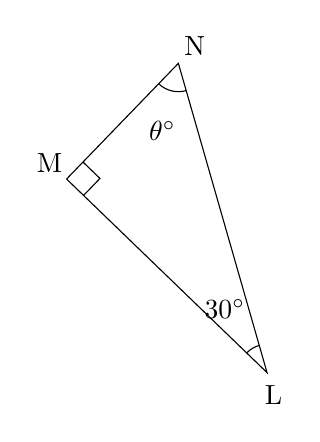
\begin{tikzpicture}[scale=1.2, baseline=(current bounding box.north)]

    \begin{scope}[rotate=106]
      \coordinate (A) at (0,0);
      \coordinate (B) at (3.4049428295605413,0);
      \coordinate (C) at (intersection cs: first line={(A)--($(A)+(30:4cm)$)}, second line={(B)--($(B)+(180-60:4cm)$)});
      \draw (A) -- (B) -- (C) -- cycle;

      % Mark angles with arcs
      \draw ($(A)!0.3cm!(B)$) arc [start angle=0, end angle=30, radius=0.3cm];
      \draw ($(B)!0.3cm!(C)$) arc [start angle=180-60, end angle=180, radius=0.3cm];
      % \draw ($(C)!0.3cm!(A)$) arc [start angle=180+30, end angle=360-60, radius=0.3cm];
      % rt angle mark at C
      % \tkzMarkRightAng0le(A,C,B); % uses \usepackage{tkz-euclide}
      \draw ($(C)!0.25cm!(A)$) -- ($(C)!0.25cm!(A)!0.25cm!90:(A)$) -- ($(C)!0.25cm!(B)$);
      %  The ($(C)!0.3cm!(A)!0.3cm!90:(A)$) syntax is used to specify a point that is 0.3cm away from the point ($(C)!0.3cm!(A)$) in a direction that is perpendicular to the line connecting points C and A. This is achieved by first specifying the point ($(C)!0.3cm!(A)$) and then rotating it by 90 degrees around point A using the !angle:anchor syntax.

      % Label angles
      \node at ($(A)!-0.25cm!(B)$) {L};
      \node at ($(B)!-0.25cm!(C)$) {N};
      \node at ($(C)!-0.25cm!(A)$) {M};

      % Mark angles in degrees
      \coordinate (midBC) at ($(B)!0.5!(C)$);
      \node at ($(A)!0.665cm!(midBC)!0.15cm!(C)$) {$30^\circ$};

      \coordinate (midAC) at ($(A)!0.5!(C)$);
      \node at ($(B)!0.65cm!(midAC)!0.15cm!(C)$) {$\theta^\circ$};

      % \coordinate (midAB) at ($(A)!0.5!(B)$);
      % \node at ($(C)!0.55cm!(midAB)$) {<<angleCValueDisplay>>$^\circ$};

    \end{scope}
  \end{tikzpicture}
\end{minipage}%
\hfill
\begin{minipage}{0.4\textwidth}
  \begin{align*}
    \theta^\circ &= 90^\circ - \angle \text{\dotuline{~~~~~~~}} \\
    &= 90^\circ - \dotuline{~~~~~~~}^\circ  \\
    &= \dotuline{~~~~~~~}^\circ
  \end{align*}
\end{minipage}
\vspace{1cm}\begin{minipage}{0.55\textwidth}
  \refstepcounter{minipagecount}
  \noindent{(\theminipagecount)}\quad
  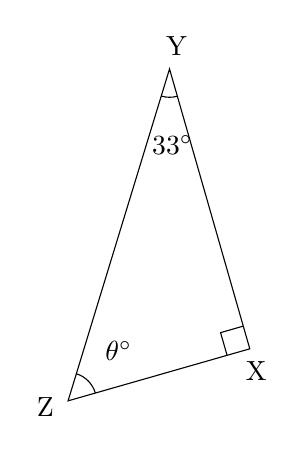
\begin{tikzpicture}[scale=1.2, baseline=(current bounding box.north)]

    \begin{scope}[rotate=253]
      \coordinate (A) at (0,0);
      \coordinate (B) at (3.6727950186846243,0);
      \coordinate (C) at (intersection cs: first line={(A)--($(A)+(33:4cm)$)}, second line={(B)--($(B)+(180-57:4cm)$)});
      \draw (A) -- (B) -- (C) -- cycle;

      % Mark angles with arcs
      \draw ($(A)!0.3cm!(B)$) arc [start angle=0, end angle=33, radius=0.3cm];
      \draw ($(B)!0.3cm!(C)$) arc [start angle=180-57, end angle=180, radius=0.3cm];
      % \draw ($(C)!0.3cm!(A)$) arc [start angle=180+33, end angle=360-57, radius=0.3cm];
      % rt angle mark at C
      % \tkzMarkRightAng0le(A,C,B); % uses \usepackage{tkz-euclide}
      \draw ($(C)!0.25cm!(A)$) -- ($(C)!0.25cm!(A)!0.25cm!90:(A)$) -- ($(C)!0.25cm!(B)$);
      %  The ($(C)!0.3cm!(A)!0.3cm!90:(A)$) syntax is used to specify a point that is 0.3cm away from the point ($(C)!0.3cm!(A)$) in a direction that is perpendicular to the line connecting points C and A. This is achieved by first specifying the point ($(C)!0.3cm!(A)$) and then rotating it by 90 degrees around point A using the !angle:anchor syntax.

      % Label angles
      \node at ($(A)!-0.25cm!(B)$) {Y};
      \node at ($(B)!-0.25cm!(C)$) {Z};
      \node at ($(C)!-0.25cm!(A)$) {X};

      % Mark angles in degrees
      \coordinate (midBC) at ($(B)!0.5!(C)$);
      \node at ($(A)!0.665cm!(midBC)!0.15cm!(C)$) {$33^\circ$};

      \coordinate (midAC) at ($(A)!0.5!(C)$);
      \node at ($(B)!0.65cm!(midAC)!0.15cm!(C)$) {$\theta^\circ$};

      % \coordinate (midAB) at ($(A)!0.5!(B)$);
      % \node at ($(C)!0.55cm!(midAB)$) {<<angleCValueDisplay>>$^\circ$};

    \end{scope}
  \end{tikzpicture}
\end{minipage}%
\hfill
\begin{minipage}{0.4\textwidth}
  \begin{align*}
    \theta^\circ &= 90^\circ - \angle \text{\dotuline{~~~~~~~}} \\
    &= 90^\circ - \dotuline{~~~~~~~}^\circ  \\
    &= \dotuline{~~~~~~~}^\circ
  \end{align*}
\end{minipage}
\vspace{1cm}\begin{minipage}{0.55\textwidth}
  \refstepcounter{minipagecount}
  \noindent{(\theminipagecount)}\quad
  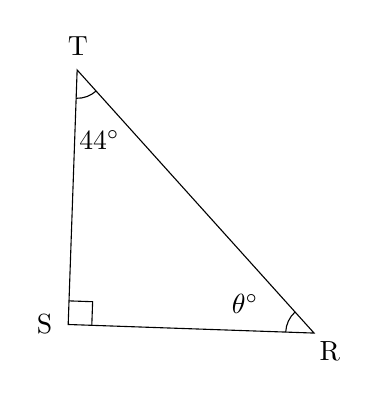
\begin{tikzpicture}[scale=1.2, baseline=(current bounding box.north)]

    \begin{scope}[rotate=132]
      \coordinate (A) at (0,0);
      \coordinate (B) at (3.7466669839293196,0);
      \coordinate (C) at (intersection cs: first line={(A)--($(A)+(46:4cm)$)}, second line={(B)--($(B)+(180-44:4cm)$)});
      \draw (A) -- (B) -- (C) -- cycle;

      % Mark angles with arcs
      \draw ($(A)!0.3cm!(B)$) arc [start angle=0, end angle=46, radius=0.3cm];
      \draw ($(B)!0.3cm!(C)$) arc [start angle=180-44, end angle=180, radius=0.3cm];
      % \draw ($(C)!0.3cm!(A)$) arc [start angle=180+46, end angle=360-44, radius=0.3cm];
      % rt angle mark at C
      % \tkzMarkRightAng0le(A,C,B); % uses \usepackage{tkz-euclide}
      \draw ($(C)!0.25cm!(A)$) -- ($(C)!0.25cm!(A)!0.25cm!90:(A)$) -- ($(C)!0.25cm!(B)$);
      %  The ($(C)!0.3cm!(A)!0.3cm!90:(A)$) syntax is used to specify a point that is 0.3cm away from the point ($(C)!0.3cm!(A)$) in a direction that is perpendicular to the line connecting points C and A. This is achieved by first specifying the point ($(C)!0.3cm!(A)$) and then rotating it by 90 degrees around point A using the !angle:anchor syntax.

      % Label angles
      \node at ($(A)!-0.25cm!(B)$) {R};
      \node at ($(B)!-0.25cm!(C)$) {T};
      \node at ($(C)!-0.25cm!(A)$) {S};

      % Mark angles in degrees
      \coordinate (midBC) at ($(B)!0.5!(C)$);
      \node at ($(A)!0.665cm!(midBC)!0.15cm!(C)$) {$\theta^\circ$};

      \coordinate (midAC) at ($(A)!0.5!(C)$);
      \node at ($(B)!0.65cm!(midAC)!0.15cm!(C)$) {$44^\circ$};

      % \coordinate (midAB) at ($(A)!0.5!(B)$);
      % \node at ($(C)!0.55cm!(midAB)$) {<<angleCValueDisplay>>$^\circ$};

    \end{scope}
  \end{tikzpicture}
\end{minipage}%
\hfill
\begin{minipage}{0.4\textwidth}
  \begin{align*}
    \theta^\circ &= 90^\circ - \angle \text{\dotuline{~~~~~~~}} \\
    &= 90^\circ - \dotuline{~~~~~~~}^\circ  \\
    &= \dotuline{~~~~~~~}^\circ
  \end{align*}
\end{minipage}
\vspace{1cm}\begin{minipage}{0.55\textwidth}
  \refstepcounter{minipagecount}
  \noindent{(\theminipagecount)}\quad
  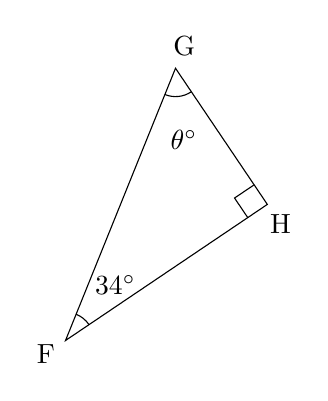
\begin{tikzpicture}[scale=1.2, baseline=(current bounding box.north)]

    \begin{scope}[rotate=248]
      \coordinate (A) at (0,0);
      \coordinate (B) at (3.1072000382861087,0);
      \coordinate (C) at (intersection cs: first line={(A)--($(A)+(56:4cm)$)}, second line={(B)--($(B)+(180-34:4cm)$)});
      \draw (A) -- (B) -- (C) -- cycle;

      % Mark angles with arcs
      \draw ($(A)!0.3cm!(B)$) arc [start angle=0, end angle=56, radius=0.3cm];
      \draw ($(B)!0.3cm!(C)$) arc [start angle=180-34, end angle=180, radius=0.3cm];
      % \draw ($(C)!0.3cm!(A)$) arc [start angle=180+56, end angle=360-34, radius=0.3cm];
      % rt angle mark at C
      % \tkzMarkRightAng0le(A,C,B); % uses \usepackage{tkz-euclide}
      \draw ($(C)!0.25cm!(A)$) -- ($(C)!0.25cm!(A)!0.25cm!90:(A)$) -- ($(C)!0.25cm!(B)$);
      %  The ($(C)!0.3cm!(A)!0.3cm!90:(A)$) syntax is used to specify a point that is 0.3cm away from the point ($(C)!0.3cm!(A)$) in a direction that is perpendicular to the line connecting points C and A. This is achieved by first specifying the point ($(C)!0.3cm!(A)$) and then rotating it by 90 degrees around point A using the !angle:anchor syntax.

      % Label angles
      \node at ($(A)!-0.25cm!(B)$) {G};
      \node at ($(B)!-0.25cm!(C)$) {F};
      \node at ($(C)!-0.25cm!(A)$) {H};

      % Mark angles in degrees
      \coordinate (midBC) at ($(B)!0.5!(C)$);
      \node at ($(A)!0.665cm!(midBC)!0.15cm!(C)$) {$\theta^\circ$};

      \coordinate (midAC) at ($(A)!0.5!(C)$);
      \node at ($(B)!0.65cm!(midAC)!0.15cm!(C)$) {$34^\circ$};

      % \coordinate (midAB) at ($(A)!0.5!(B)$);
      % \node at ($(C)!0.55cm!(midAB)$) {<<angleCValueDisplay>>$^\circ$};

    \end{scope}
  \end{tikzpicture}
\end{minipage}%
\hfill
\begin{minipage}{0.4\textwidth}
  \begin{align*}
    \theta^\circ &= 90^\circ - \angle \text{\dotuline{~~~~~~~}} \\
    &= 90^\circ - \dotuline{~~~~~~~}^\circ  \\
    &= \dotuline{~~~~~~~}^\circ
  \end{align*}
\end{minipage}
\vspace{1cm}\begin{minipage}{0.55\textwidth}
  \refstepcounter{minipagecount}
  \noindent{(\theminipagecount)}\quad
  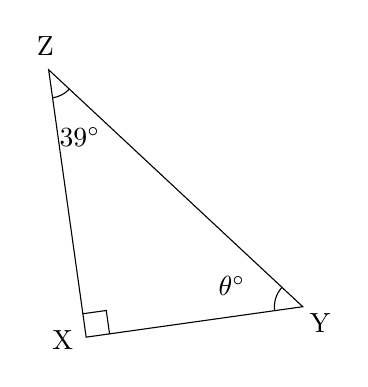
\begin{tikzpicture}[scale=1.2, baseline=(current bounding box.north)]

    \begin{scope}[rotate=137]
      \coordinate (A) at (0,0);
      \coordinate (B) at (3.6768811932272447,0);
      \coordinate (C) at (intersection cs: first line={(A)--($(A)+(51:4cm)$)}, second line={(B)--($(B)+(180-39:4cm)$)});
      \draw (A) -- (B) -- (C) -- cycle;

      % Mark angles with arcs
      \draw ($(A)!0.3cm!(B)$) arc [start angle=0, end angle=51, radius=0.3cm];
      \draw ($(B)!0.3cm!(C)$) arc [start angle=180-39, end angle=180, radius=0.3cm];
      % \draw ($(C)!0.3cm!(A)$) arc [start angle=180+51, end angle=360-39, radius=0.3cm];
      % rt angle mark at C
      % \tkzMarkRightAng0le(A,C,B); % uses \usepackage{tkz-euclide}
      \draw ($(C)!0.25cm!(A)$) -- ($(C)!0.25cm!(A)!0.25cm!90:(A)$) -- ($(C)!0.25cm!(B)$);
      %  The ($(C)!0.3cm!(A)!0.3cm!90:(A)$) syntax is used to specify a point that is 0.3cm away from the point ($(C)!0.3cm!(A)$) in a direction that is perpendicular to the line connecting points C and A. This is achieved by first specifying the point ($(C)!0.3cm!(A)$) and then rotating it by 90 degrees around point A using the !angle:anchor syntax.

      % Label angles
      \node at ($(A)!-0.25cm!(B)$) {Y};
      \node at ($(B)!-0.25cm!(C)$) {Z};
      \node at ($(C)!-0.25cm!(A)$) {X};

      % Mark angles in degrees
      \coordinate (midBC) at ($(B)!0.5!(C)$);
      \node at ($(A)!0.665cm!(midBC)!0.15cm!(C)$) {$\theta^\circ$};

      \coordinate (midAC) at ($(A)!0.5!(C)$);
      \node at ($(B)!0.65cm!(midAC)!0.15cm!(C)$) {$39^\circ$};

      % \coordinate (midAB) at ($(A)!0.5!(B)$);
      % \node at ($(C)!0.55cm!(midAB)$) {<<angleCValueDisplay>>$^\circ$};

    \end{scope}
  \end{tikzpicture}
\end{minipage}%
\hfill
\begin{minipage}{0.4\textwidth}
  \begin{align*}
    \theta^\circ &= 90^\circ - \angle \text{\dotuline{~~~~~~~}} \\
    &= 90^\circ - \dotuline{~~~~~~~}^\circ  \\
    &= \dotuline{~~~~~~~}^\circ
  \end{align*}
\end{minipage}
\vspace{1cm}\begin{minipage}{0.55\textwidth}
  \refstepcounter{minipagecount}
  \noindent{(\theminipagecount)}\quad
  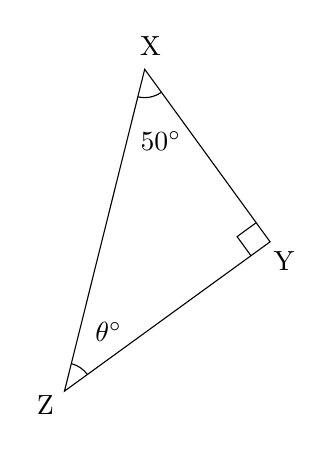
\begin{tikzpicture}[scale=1.2, baseline=(current bounding box.north)]

    \begin{scope}[rotate=256]
      \coordinate (A) at (0,0);
      \coordinate (B) at (3.510335498912445,0);
      \coordinate (C) at (intersection cs: first line={(A)--($(A)+(50:4cm)$)}, second line={(B)--($(B)+(180-40:4cm)$)});
      \draw (A) -- (B) -- (C) -- cycle;

      % Mark angles with arcs
      \draw ($(A)!0.3cm!(B)$) arc [start angle=0, end angle=50, radius=0.3cm];
      \draw ($(B)!0.3cm!(C)$) arc [start angle=180-40, end angle=180, radius=0.3cm];
      % \draw ($(C)!0.3cm!(A)$) arc [start angle=180+50, end angle=360-40, radius=0.3cm];
      % rt angle mark at C
      % \tkzMarkRightAng0le(A,C,B); % uses \usepackage{tkz-euclide}
      \draw ($(C)!0.25cm!(A)$) -- ($(C)!0.25cm!(A)!0.25cm!90:(A)$) -- ($(C)!0.25cm!(B)$);
      %  The ($(C)!0.3cm!(A)!0.3cm!90:(A)$) syntax is used to specify a point that is 0.3cm away from the point ($(C)!0.3cm!(A)$) in a direction that is perpendicular to the line connecting points C and A. This is achieved by first specifying the point ($(C)!0.3cm!(A)$) and then rotating it by 90 degrees around point A using the !angle:anchor syntax.

      % Label angles
      \node at ($(A)!-0.25cm!(B)$) {X};
      \node at ($(B)!-0.25cm!(C)$) {Z};
      \node at ($(C)!-0.25cm!(A)$) {Y};

      % Mark angles in degrees
      \coordinate (midBC) at ($(B)!0.5!(C)$);
      \node at ($(A)!0.665cm!(midBC)!0.15cm!(C)$) {$50^\circ$};

      \coordinate (midAC) at ($(A)!0.5!(C)$);
      \node at ($(B)!0.65cm!(midAC)!0.15cm!(C)$) {$\theta^\circ$};

      % \coordinate (midAB) at ($(A)!0.5!(B)$);
      % \node at ($(C)!0.55cm!(midAB)$) {<<angleCValueDisplay>>$^\circ$};

    \end{scope}
  \end{tikzpicture}
\end{minipage}%
\hfill
\begin{minipage}{0.4\textwidth}
  \begin{align*}
    \theta^\circ &= 90^\circ - \angle \text{\dotuline{~~~~~~~}} \\
    &= 90^\circ - \dotuline{~~~~~~~}^\circ  \\
    &= \dotuline{~~~~~~~}^\circ
  \end{align*}
\end{minipage}
\vspace{1cm}\begin{minipage}{0.55\textwidth}
  \refstepcounter{minipagecount}
  \noindent{(\theminipagecount)}\quad
  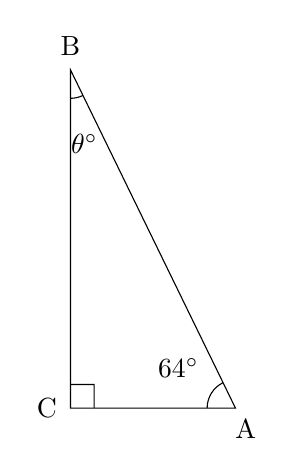
\begin{tikzpicture}[scale=1.2, baseline=(current bounding box.north)]

    \begin{scope}[rotate=116]
      \coordinate (A) at (0,0);
      \coordinate (B) at (3.9815020108396078,0);
      \coordinate (C) at (intersection cs: first line={(A)--($(A)+(64:4cm)$)}, second line={(B)--($(B)+(180-26:4cm)$)});
      \draw (A) -- (B) -- (C) -- cycle;

      % Mark angles with arcs
      \draw ($(A)!0.3cm!(B)$) arc [start angle=0, end angle=64, radius=0.3cm];
      \draw ($(B)!0.3cm!(C)$) arc [start angle=180-26, end angle=180, radius=0.3cm];
      % \draw ($(C)!0.3cm!(A)$) arc [start angle=180+64, end angle=360-26, radius=0.3cm];
      % rt angle mark at C
      % \tkzMarkRightAng0le(A,C,B); % uses \usepackage{tkz-euclide}
      \draw ($(C)!0.25cm!(A)$) -- ($(C)!0.25cm!(A)!0.25cm!90:(A)$) -- ($(C)!0.25cm!(B)$);
      %  The ($(C)!0.3cm!(A)!0.3cm!90:(A)$) syntax is used to specify a point that is 0.3cm away from the point ($(C)!0.3cm!(A)$) in a direction that is perpendicular to the line connecting points C and A. This is achieved by first specifying the point ($(C)!0.3cm!(A)$) and then rotating it by 90 degrees around point A using the !angle:anchor syntax.

      % Label angles
      \node at ($(A)!-0.25cm!(B)$) {A};
      \node at ($(B)!-0.25cm!(C)$) {B};
      \node at ($(C)!-0.25cm!(A)$) {C};

      % Mark angles in degrees
      \coordinate (midBC) at ($(B)!0.5!(C)$);
      \node at ($(A)!0.665cm!(midBC)!0.15cm!(C)$) {$64^\circ$};

      \coordinate (midAC) at ($(A)!0.5!(C)$);
      \node at ($(B)!0.65cm!(midAC)!0.15cm!(C)$) {$\theta^\circ$};

      % \coordinate (midAB) at ($(A)!0.5!(B)$);
      % \node at ($(C)!0.55cm!(midAB)$) {<<angleCValueDisplay>>$^\circ$};

    \end{scope}
  \end{tikzpicture}
\end{minipage}%
\hfill
\begin{minipage}{0.4\textwidth}
  \begin{align*}
    \theta^\circ &= 90^\circ - \angle \text{\dotuline{~~~~~~~}} \\
    &= 90^\circ - \dotuline{~~~~~~~}^\circ  \\
    &= \dotuline{~~~~~~~}^\circ
  \end{align*}
\end{minipage}
\vspace{1cm}\begin{minipage}{0.55\textwidth}
  \refstepcounter{minipagecount}
  \noindent{(\theminipagecount)}\quad
  \begin{tikzpicture}[scale=1.2, baseline=(current bounding box.north)]

    \begin{scope}[rotate=80]
      \coordinate (A) at (0,0);
      \coordinate (B) at (3.853088967381318,0);
      \coordinate (C) at (intersection cs: first line={(A)--($(A)+(52:4cm)$)}, second line={(B)--($(B)+(180-38:4cm)$)});
      \draw (A) -- (B) -- (C) -- cycle;

      % Mark angles with arcs
      \draw ($(A)!0.3cm!(B)$) arc [start angle=0, end angle=52, radius=0.3cm];
      \draw ($(B)!0.3cm!(C)$) arc [start angle=180-38, end angle=180, radius=0.3cm];
      % \draw ($(C)!0.3cm!(A)$) arc [start angle=180+52, end angle=360-38, radius=0.3cm];
      % rt angle mark at C
      % \tkzMarkRightAng0le(A,C,B); % uses \usepackage{tkz-euclide}
      \draw ($(C)!0.25cm!(A)$) -- ($(C)!0.25cm!(A)!0.25cm!90:(A)$) -- ($(C)!0.25cm!(B)$);
      %  The ($(C)!0.3cm!(A)!0.3cm!90:(A)$) syntax is used to specify a point that is 0.3cm away from the point ($(C)!0.3cm!(A)$) in a direction that is perpendicular to the line connecting points C and A. This is achieved by first specifying the point ($(C)!0.3cm!(A)$) and then rotating it by 90 degrees around point A using the !angle:anchor syntax.

      % Label angles
      \node at ($(A)!-0.25cm!(B)$) {M};
      \node at ($(B)!-0.25cm!(C)$) {L};
      \node at ($(C)!-0.25cm!(A)$) {N};

      % Mark angles in degrees
      \coordinate (midBC) at ($(B)!0.5!(C)$);
      \node at ($(A)!0.665cm!(midBC)!0.15cm!(C)$) {$\theta^\circ$};

      \coordinate (midAC) at ($(A)!0.5!(C)$);
      \node at ($(B)!0.65cm!(midAC)!0.15cm!(C)$) {$38^\circ$};

      % \coordinate (midAB) at ($(A)!0.5!(B)$);
      % \node at ($(C)!0.55cm!(midAB)$) {<<angleCValueDisplay>>$^\circ$};

    \end{scope}
  \end{tikzpicture}
\end{minipage}%
\hfill
\begin{minipage}{0.4\textwidth}
  \begin{align*}
    \theta^\circ &= 90^\circ - \angle \text{\dotuline{~~~~~~~}} \\
    &= 90^\circ - \dotuline{~~~~~~~}^\circ  \\
    &= \dotuline{~~~~~~~}^\circ
  \end{align*}
\end{minipage}
\vspace{1cm}\begin{minipage}{0.55\textwidth}
  \refstepcounter{minipagecount}
  \noindent{(\theminipagecount)}\quad
  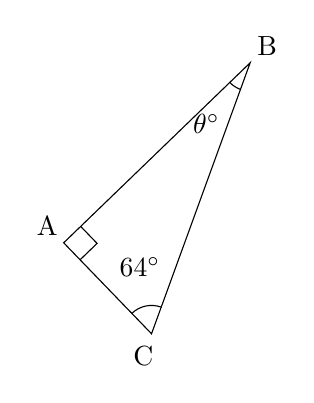
\begin{tikzpicture}[scale=1.2, baseline=(current bounding box.north)]

    \begin{scope}[rotate=70]
      \coordinate (A) at (0,0);
      \coordinate (B) at (3.0519153042160743,0);
      \coordinate (C) at (intersection cs: first line={(A)--($(A)+(64:4cm)$)}, second line={(B)--($(B)+(180-26:4cm)$)});
      \draw (A) -- (B) -- (C) -- cycle;

      % Mark angles with arcs
      \draw ($(A)!0.3cm!(B)$) arc [start angle=0, end angle=64, radius=0.3cm];
      \draw ($(B)!0.3cm!(C)$) arc [start angle=180-26, end angle=180, radius=0.3cm];
      % \draw ($(C)!0.3cm!(A)$) arc [start angle=180+64, end angle=360-26, radius=0.3cm];
      % rt angle mark at C
      % \tkzMarkRightAng0le(A,C,B); % uses \usepackage{tkz-euclide}
      \draw ($(C)!0.25cm!(A)$) -- ($(C)!0.25cm!(A)!0.25cm!90:(A)$) -- ($(C)!0.25cm!(B)$);
      %  The ($(C)!0.3cm!(A)!0.3cm!90:(A)$) syntax is used to specify a point that is 0.3cm away from the point ($(C)!0.3cm!(A)$) in a direction that is perpendicular to the line connecting points C and A. This is achieved by first specifying the point ($(C)!0.3cm!(A)$) and then rotating it by 90 degrees around point A using the !angle:anchor syntax.

      % Label angles
      \node at ($(A)!-0.25cm!(B)$) {C};
      \node at ($(B)!-0.25cm!(C)$) {B};
      \node at ($(C)!-0.25cm!(A)$) {A};

      % Mark angles in degrees
      \coordinate (midBC) at ($(B)!0.5!(C)$);
      \node at ($(A)!0.665cm!(midBC)!0.15cm!(C)$) {$64^\circ$};

      \coordinate (midAC) at ($(A)!0.5!(C)$);
      \node at ($(B)!0.65cm!(midAC)!0.15cm!(C)$) {$\theta^\circ$};

      % \coordinate (midAB) at ($(A)!0.5!(B)$);
      % \node at ($(C)!0.55cm!(midAB)$) {<<angleCValueDisplay>>$^\circ$};

    \end{scope}
  \end{tikzpicture}
\end{minipage}%
\hfill
\begin{minipage}{0.4\textwidth}
  \begin{align*}
    \theta^\circ &= 90^\circ - \angle \text{\dotuline{~~~~~~~}} \\
    &= 90^\circ - \dotuline{~~~~~~~}^\circ  \\
    &= \dotuline{~~~~~~~}^\circ
  \end{align*}
\end{minipage}
\vspace{1cm}\begin{minipage}{0.55\textwidth}
  \refstepcounter{minipagecount}
  \noindent{(\theminipagecount)}\quad
  \begin{tikzpicture}[scale=1.2, baseline=(current bounding box.north)]

    \begin{scope}[rotate=57]
      \coordinate (A) at (0,0);
      \coordinate (B) at (3.7290561349628053,0);
      \coordinate (C) at (intersection cs: first line={(A)--($(A)+(47:4cm)$)}, second line={(B)--($(B)+(180-43:4cm)$)});
      \draw (A) -- (B) -- (C) -- cycle;

      % Mark angles with arcs
      \draw ($(A)!0.3cm!(B)$) arc [start angle=0, end angle=47, radius=0.3cm];
      \draw ($(B)!0.3cm!(C)$) arc [start angle=180-43, end angle=180, radius=0.3cm];
      % \draw ($(C)!0.3cm!(A)$) arc [start angle=180+47, end angle=360-43, radius=0.3cm];
      % rt angle mark at C
      % \tkzMarkRightAng0le(A,C,B); % uses \usepackage{tkz-euclide}
      \draw ($(C)!0.25cm!(A)$) -- ($(C)!0.25cm!(A)!0.25cm!90:(A)$) -- ($(C)!0.25cm!(B)$);
      %  The ($(C)!0.3cm!(A)!0.3cm!90:(A)$) syntax is used to specify a point that is 0.3cm away from the point ($(C)!0.3cm!(A)$) in a direction that is perpendicular to the line connecting points C and A. This is achieved by first specifying the point ($(C)!0.3cm!(A)$) and then rotating it by 90 degrees around point A using the !angle:anchor syntax.

      % Label angles
      \node at ($(A)!-0.25cm!(B)$) {X};
      \node at ($(B)!-0.25cm!(C)$) {Z};
      \node at ($(C)!-0.25cm!(A)$) {Y};

      % Mark angles in degrees
      \coordinate (midBC) at ($(B)!0.5!(C)$);
      \node at ($(A)!0.665cm!(midBC)!0.15cm!(C)$) {$47^\circ$};

      \coordinate (midAC) at ($(A)!0.5!(C)$);
      \node at ($(B)!0.65cm!(midAC)!0.15cm!(C)$) {$\theta^\circ$};

      % \coordinate (midAB) at ($(A)!0.5!(B)$);
      % \node at ($(C)!0.55cm!(midAB)$) {<<angleCValueDisplay>>$^\circ$};

    \end{scope}
  \end{tikzpicture}
\end{minipage}%
\hfill
\begin{minipage}{0.4\textwidth}
  \begin{align*}
    \theta^\circ &= 90^\circ - \angle \text{\dotuline{~~~~~~~}} \\
    &= 90^\circ - \dotuline{~~~~~~~}^\circ  \\
    &= \dotuline{~~~~~~~}^\circ
  \end{align*}
\end{minipage}
\vspace{1cm}\begin{minipage}{0.55\textwidth}
  \refstepcounter{minipagecount}
  \noindent{(\theminipagecount)}\quad
  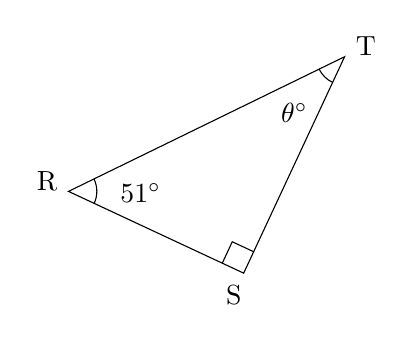
\begin{tikzpicture}[scale=1.2, baseline=(current bounding box.north)]

    \begin{scope}[rotate=206]
      \coordinate (A) at (0,0);
      \coordinate (B) at (3.2510534965258704,0);
      \coordinate (C) at (intersection cs: first line={(A)--($(A)+(39:4cm)$)}, second line={(B)--($(B)+(180-51:4cm)$)});
      \draw (A) -- (B) -- (C) -- cycle;

      % Mark angles with arcs
      \draw ($(A)!0.3cm!(B)$) arc [start angle=0, end angle=39, radius=0.3cm];
      \draw ($(B)!0.3cm!(C)$) arc [start angle=180-51, end angle=180, radius=0.3cm];
      % \draw ($(C)!0.3cm!(A)$) arc [start angle=180+39, end angle=360-51, radius=0.3cm];
      % rt angle mark at C
      % \tkzMarkRightAng0le(A,C,B); % uses \usepackage{tkz-euclide}
      \draw ($(C)!0.25cm!(A)$) -- ($(C)!0.25cm!(A)!0.25cm!90:(A)$) -- ($(C)!0.25cm!(B)$);
      %  The ($(C)!0.3cm!(A)!0.3cm!90:(A)$) syntax is used to specify a point that is 0.3cm away from the point ($(C)!0.3cm!(A)$) in a direction that is perpendicular to the line connecting points C and A. This is achieved by first specifying the point ($(C)!0.3cm!(A)$) and then rotating it by 90 degrees around point A using the !angle:anchor syntax.

      % Label angles
      \node at ($(A)!-0.25cm!(B)$) {T};
      \node at ($(B)!-0.25cm!(C)$) {R};
      \node at ($(C)!-0.25cm!(A)$) {S};

      % Mark angles in degrees
      \coordinate (midBC) at ($(B)!0.5!(C)$);
      \node at ($(A)!0.665cm!(midBC)!0.15cm!(C)$) {$\theta^\circ$};

      \coordinate (midAC) at ($(A)!0.5!(C)$);
      \node at ($(B)!0.65cm!(midAC)!0.15cm!(C)$) {$51^\circ$};

      % \coordinate (midAB) at ($(A)!0.5!(B)$);
      % \node at ($(C)!0.55cm!(midAB)$) {<<angleCValueDisplay>>$^\circ$};

    \end{scope}
  \end{tikzpicture}
\end{minipage}%
\hfill
\begin{minipage}{0.4\textwidth}
  \begin{align*}
    \theta^\circ &= 90^\circ - \angle \text{\dotuline{~~~~~~~}} \\
    &= 90^\circ - \dotuline{~~~~~~~}^\circ  \\
    &= \dotuline{~~~~~~~}^\circ
  \end{align*}
\end{minipage}
\vspace{1cm}

\end{document}
